\section{Samples \label{sec:samples}}

Data collected with the CMS detector during 2012 running at an energy of $\sqrt{s}=8$~TeV are searched. The data collection was split into four periods labeled A, B, C, and D.
All data collected by CMS undergo a prompt reconstruction as described in section~\ref{sec:computing}. The first two run periods, A and B, underwent an additional
re-reconstruction so as to have the latest reconstruction improvements and calibration constants. The re-reconstructed samples are used for the A and B periods while the promptly
reconstructed samples are used for the C and D periods.

CMS has a Data Certification team which checks all data collected and certifies the data as good for analysis. The certification requires all detector subsystems to be
operating at full ability, or at least close enough to full ability to not have a detrimental effect on offline analyses. Additionally, higher level objects such as muons
and electrons are checked to make sure the data are good for physics analyses. For this particular analysis, the RPC trigger plays an important role, as discussed in
section~\ref{sec:computing}, and so the RPC is required to be included in the L1 trigger for all data searched. This leads to the searches using slightly less data
than most other CMS analyses on 2012 data. The data sample used by this analysis corresponds to 18.8~fb$^{-1}$.

Multiple different signal Monte Carlo (MC) simulation samples are produced to account for the different signatures an HSCP could have;
more detail on the signal models can be found in Sec.~\ref{sec:BSM}.

Pair production of strongly--interacting gluino and stop samples are produced with
masses in the range 300--1500~GeV$/c^2$ and 100--1000~GeV$/c^2$, respectively.
The gluinos are generated in the split SUSY scenario~\cite{ArkaniHamed:2004fb, Giudice:2004tc}
under the assumption of high squark masses of 10~TeV. The samples are generated using PYTHIAv8.153~\cite{Sjostrand:2007gs}.
Samples are produced with the fraction $f$ of gluinos forming neutral glueball $R$-hadrons set to $f=1.0$, 0.5, and 0.1.
%The value of $f=1.0$ results in all gluino $R$-hadrons being produced neutral.
%, the \muononly\ analysis is designed to still have sensitivity in this case.
The samples are also produced with two different modelings of the nuclear interaction of R-hadrons with matter: the cloud interaction and charge suppressed models.
The charge suppressed model results in all $R$-hadrons being neutral after a nuclear interaction while the cloud interaction model allows for $R$-hadrons
to be charged or neutral after a nuclear interaction.
The cloud interaction model should be assumed for samples unless explicitly stated otherwise.
Most HSCP will not have a nuclear interaction while passing through the CMS tracker, however almost all of them will have such an interaction in the calorimeter.

The above effects can lead to many interesting signatures in the CMS detector. A $R$-hadron neutral after hadronization will be neutral while it traverses the silicon tracker
but may gain charge in the calorimeter under the cloud model and leave hits in the muon system. If the glueball fraction is 1.0, then this would
be the only way to detect gluino HSCP. The \muononly\ analysis is designed to have sensitivity to HSCP of this type. On the other hand HSCP produced charged under
the charge suppression model will be charged in the silicon tracker but always neutral in the muon system. The \tkonly\ analysis is designed to be sensitive
to HSCP of this type. A third signature is an HSCP charged in both the muon and tracker systems which would have a signature similar to a muon.
HSCP produced neutral under the charge suppression model would never be charged during their passage through CMS and thus are outside the scope
of the present CMS HSCP search.

The \pt, $\eta$, and $\beta$ distributions of gluino and stop particles at generation are shown in Figs.~\ref{fig:GenGluino} and~\ref{fig:GenStop}, respectively.

\begin{figure}
 \begin{center}
  \includegraphics[clip=false, trim=0.0cm 0cm 1.4cm 0cm, width=0.44\textwidth]{figures/muonly/Selection_Comp_GenGluino_genpT}
  \includegraphics[clip=false, trim=0.0cm 0cm 1.4cm 0cm, width=0.44\textwidth]{figures/muonly/Selection_Comp_GenGluino_geneta}
  \includegraphics[clip=false, trim=0.0cm 0cm 1.4cm 0cm, width=0.44\textwidth]{figures/muonly/Selection_Comp_GenGluino_genbeta}
 \end{center}
 \caption[Distribution of \pt, $\eta$, and $\beta$ for various gluino samples at generation]
{Distribution of kinematic variables for various gluino ($\tilde{g}$) samples at generation:
\pt\ (top left), $\eta$ (top right), and $\beta$ (bottom).
   \label{fig:GenGluino}}
\end{figure}

\begin{figure}
 \begin{center}
  \includegraphics[clip=false, trim=0.0cm 0cm 1.4cm 0cm, width=0.44\textwidth]{figures/muonly/Selection_Comp_GenStop_genpT}
  \includegraphics[clip=false, trim=0.0cm 0cm 1.4cm 0cm, width=0.44\textwidth]{figures/muonly/Selection_Comp_GenStop_geneta}
  \includegraphics[clip=false, trim=0.0cm 0cm 1.4cm 0cm, width=0.44\textwidth]{figures/muonly/Selection_Comp_GenStop_genbeta}
 \end{center}
 \caption[Distribution of \pt, $\eta$, and $\beta$ for various stop samples at generation]
{Distribution of kinematic variables for various stop ($\tilde{t}$) samples at generation:
\pt\ (top left), $\eta$ (top right), and $\beta$ (bottom).
   \label{fig:GenStop}}
\end{figure}

%One example of this is a neutral R-meson
%made of a a gluino, a down quark, and a down anti-quark interacting with a proton, which is composed of two up quarks

Additional samples are produced creating lepton-like HSCP. Stau pair samples
are produced under the minimal gauge-mediated supersymmetry breaking scenario~\cite{Giudice:1998bp} using the SPS7 slope~\cite{Allanach:2002nj}.
The ISASUGRA version 7.69~\cite{Paige:2003mg} program is used to set the particle mass scale and decay chains by specifying six parameters.
%Six parameters are set to specify the exact mGMSB scenario used. 
The number of messenger particles is set to three; the ratio of the mass of the messenger particles to the effective SUSY breaking mass scale is set to 2.0;
$tan \beta = 10$, this $\beta$ being the ratio of the vacuum expectation values of the neutral Higgses;
the sign of the supersymmetric Higgs mass parameter is made positive; and $c_{Grav}$ is greater than 10000.
The low number of messenger particles results in the stau being the NLSP.
The high value of $c_{Grav}$ results in the stau being long-lived, while varying $\Lambda$ from 31 to 180~TeV gives staus within a mass range of 100--557~GeV$/c^2$. 
The produced mass spectrum and decay chains are passed to PYTHIA v6.426~\cite{Sjostrand:2006za}. 
Stau production proceeds either by direct electroweak production or from the cascade
decay of other particles. Cascade decay is dominant due to the strong nature of the pair production mechanism for gluinos and squarks.
In order to give the best results while maintaining model independence, two stau samples are used: one with both direct production and production from cascade decays (CD)
and one with staus only produced through direct production (DP). The second sample is less dependent on the model parameters. The distributions
 of \pt, $\eta$, and $\beta$ at generation
are shown in Figs~\ref{fig:GenGMStau} and~\ref{fig:GenPPStau} for various CD and DP stau samples, respectively.

\begin{figure}
 \begin{center}
  \includegraphics[clip=false, trim=0.0cm 0cm 1.4cm 0cm, width=0.44\textwidth]{figures/muonly/Selection_Comp_GenGMStau_genpT}
  \includegraphics[clip=false, trim=0.0cm 0cm 1.4cm 0cm, width=0.44\textwidth]{figures/muonly/Selection_Comp_GenGMStau_geneta}
  \includegraphics[clip=false, trim=0.0cm 0cm 1.4cm 0cm, width=0.44\textwidth]{figures/muonly/Selection_Comp_GenGMStau_genbeta}
 \end{center}
 \caption[Distribution of \pt, $\eta$, and $\beta$ for various CD stau samples at generation]
{Distribution of kinematic variables for various CD stau ($\tilde{\tau}$) samples at generation:
\pt\ (top left), $\eta$ (top right), and $\beta$ (bottom)
   \label{fig:GenGMStau}}
\end{figure}

\begin{figure}
 \begin{center}
  \includegraphics[clip=false, trim=0.0cm 0cm 1.4cm 0cm, width=0.44\textwidth]{figures/muonly/Selection_Comp_GenPPStau_genpT}
  \includegraphics[clip=false, trim=0.0cm 0cm 1.4cm 0cm, width=0.44\textwidth]{figures/muonly/Selection_Comp_GenPPStau_geneta}
  \includegraphics[clip=false, trim=0.0cm 0cm 1.4cm 0cm, width=0.44\textwidth]{figures/muonly/Selection_Comp_GenPPStau_genbeta}
 \end{center}
 \caption[Distribution of \pt, $\eta$, and $\beta$ for various DP stau samples at generation]
{Distribution of kinematic variables for various DP stau ($\tilde{\tau}$) samples at generation:
\pt\ (top left), $\eta$ (top right) and $\beta$ (bottom).
   \label{fig:GenPPStau}}
\end{figure}

The last of the signal samples used is modified Drell-Yan production of long-lived leptons with different electrical charges.
In the model considered, the particles are neutral under $SU(3)_C$ and $SU(2)_L$ but still interact through $U(1)_Y$ interactions~\cite{Langacker:2011db}.
As all SM particles that reach CMS have Q equal to $1e$ or
are neutral, the possibility of HSCPs with non-unit charge is interesting. 
%Here and in the rest of this work, Q is meant to be the absolute value of the charge unless explicitly stated.
%The particles can generically be divided by whether they have Q<1e or Q>=1e.
The production of these particles is simulated with PYTHIA v6.426~\cite{Sjostrand:2006za}. 
Samples are produced with charge Q = $1e$, $2e$, $3e$, $4e$, $5e$, $6e$, $7e$, and $8e$ for masses of 
%100-500 GeV$/c^2$ for $Q=2e/3$;
100-1000~GeV$/c^2$ for $1e <= Q <= 5e$ and 200-1000~GeV$/c^2$ for $Q > 5e$.
%charge Q = 1/3, 2/3, 1, 2, 3, 4, 5, 6, 7, and 8e for masses of 100-500 GeV$/c^2$ for Q<1e, 100-1000 GeV$/c^2$ for 1e <= Q <= 5e, and 200-1000 for Q > 5e. 
%The samples can generically be divided by whether they have Q<1e or Q>=1e.
The distributions of \pt, $\eta$, and $\beta$ at generation for various charges and masses are shown in Fig.~\ref{fig:GenDY}.

\begin{figure}
 \begin{center}
  \includegraphics[clip=false, trim=0.0cm 0cm 1.4cm 0cm, width=0.44\textwidth]{figures/muonly/Selection_Comp_GenDY_genpT}
  \includegraphics[clip=false, trim=0.0cm 0cm 1.4cm 0cm, width=0.44\textwidth]{figures/muonly/Selection_Comp_GenDY_geneta}
  \includegraphics[clip=false, trim=0.0cm 0cm 1.4cm 0cm, width=0.44\textwidth]{figures/muonly/Selection_Comp_GenDY_genbeta}
 \end{center}
 \caption[Distribution of \pt, $\eta$, and $\beta$ for modified DY samples with various charges and masses at generation]
{Distribution of kinematic variables for modified DY samples with various charges and masses at generation:
\pt\ (top left), $\eta$ (top right) and $\beta$ (bottom).
}
   \label{fig:GenDY}
\end{figure}

All MC simulation events are overlaid with additional proton-proton collisions (see Section~\ref{sec:LHC}).
Weights are given to the events so that the distribution of additional collisions in the MC simulation samples matches what is observed in data.
The reconstruction of the event by CMSSW tries to identify each proton-proton collision as a separate primary vertex~\cite{2010EPJC...70.1165K}.
The distribution of the number of primary vertices found in events after the reweighting is shown in Figure~\ref{fig:PV} for data and MC simulation.
The samples shown in the figure are required to have been collected with one of the triggers detailed in Sec.~\ref{sec:trigger} and to have
passed the preselection requirements for the \muononly\ analysis (see Sec.~\ref{sec:preselection}).

\begin{figure}
  \begin{center}
      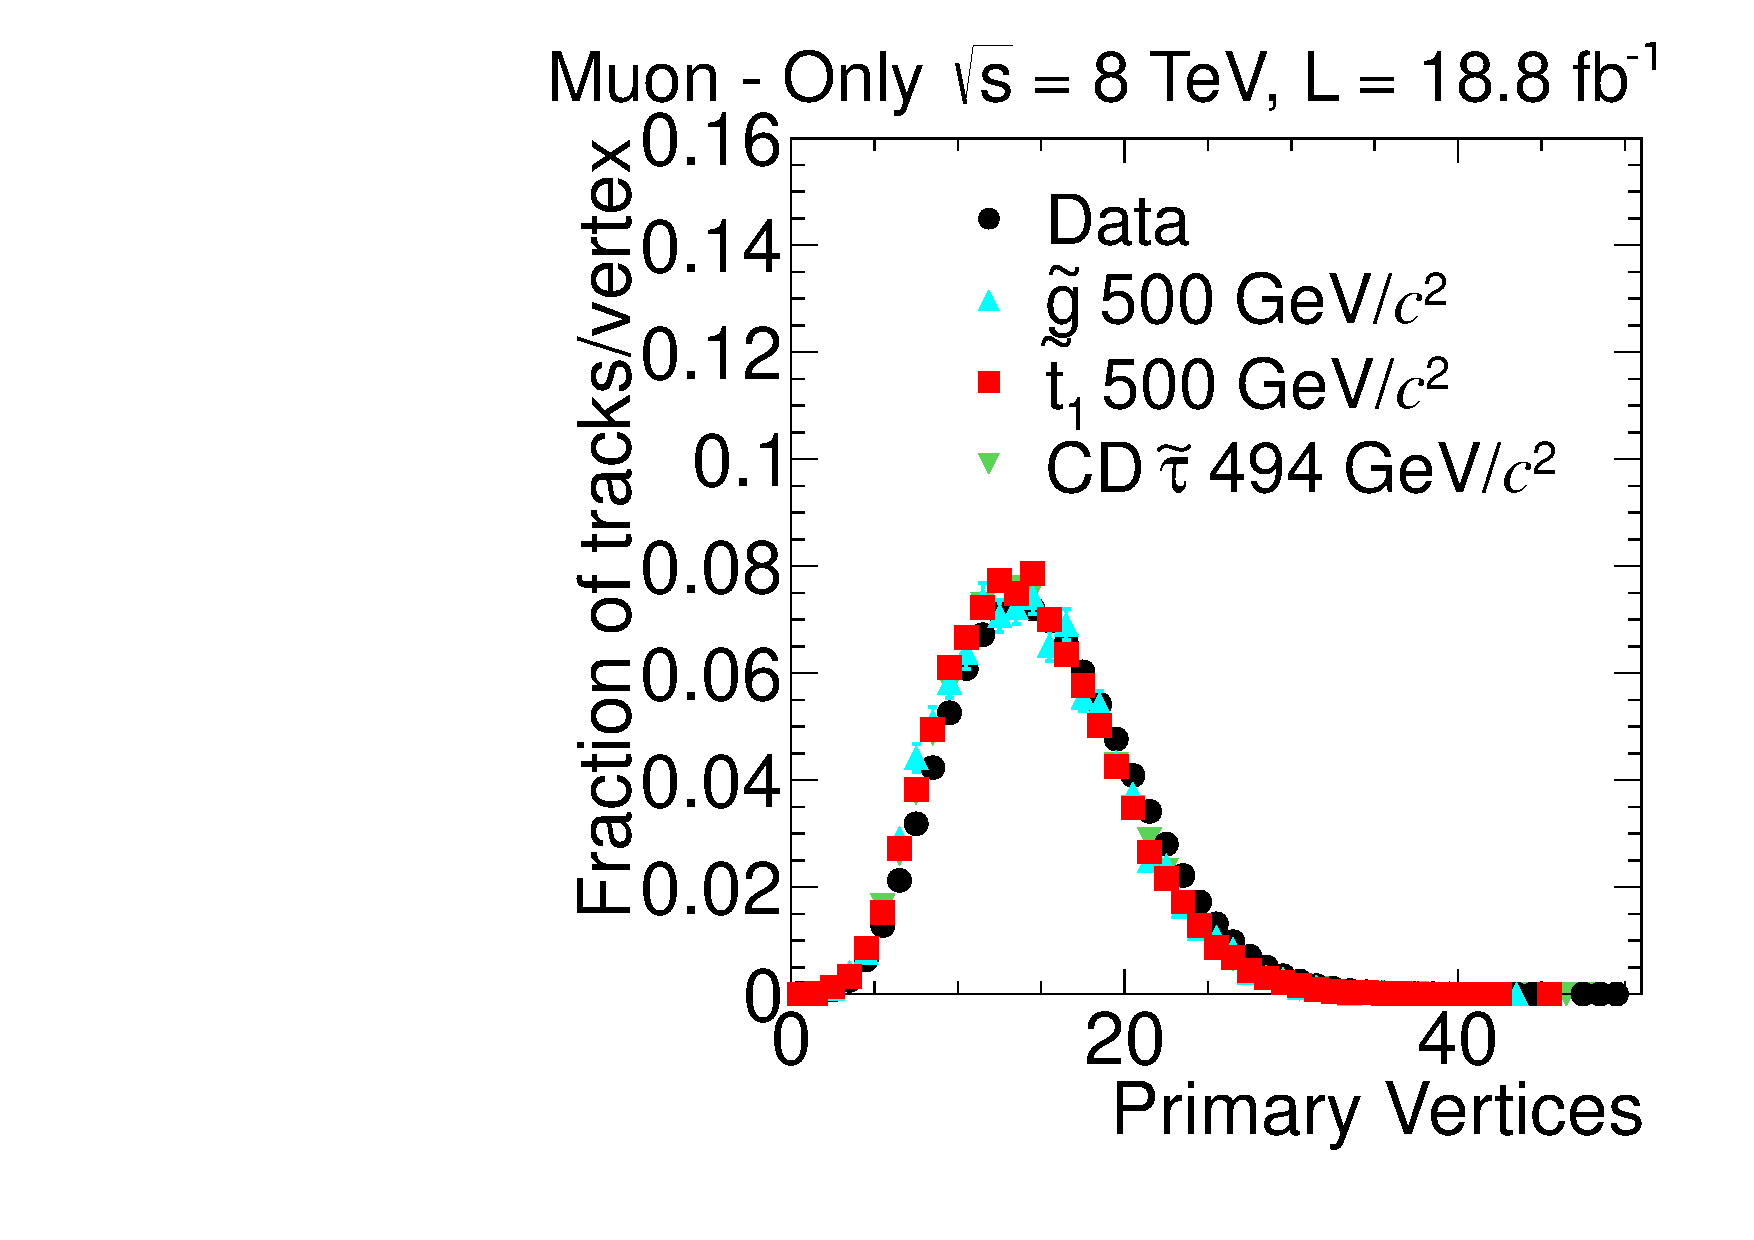
\includegraphics[clip=false, trim=0.0cm 0cm 0.0cm 0cm, width=0.44\textwidth]{figures/muonly/Selection_Comp_Signal_8TeV_PV_BS}
      \includegraphics[clip=false, trim=0.0cm 0cm 0.0cm 0cm, width=0.44\textwidth]{figures/muonly/Selection_Comp_Signal_8TeV_PVLog_BS} \\
  \end{center}
        \caption[Distribution of number of primary vertices in data and various MC simulation samples]
{Distribution of number of primary vertices in data and various MC simulation samples. 
The samples shown in the figure are required to have been collected with one of the three triggers detailed in Sec.~\ref{sec:trigger}
and to have passed the preselection criteria for the \muononly\ analysis (see Sec.~\ref{sec:preselection}).
Left with linear y-axis scale, right with log scale.
        }
      \label{fig:PV}
\end{figure}